%%%%%%%%%%%%%%%%%%%%%%%%%%%%%%%%%%%%%%%%%%%%%%%%%%%%%%%%%%%%%%%%%%%%%%%%%%%%%%%
%     STYLE POUR LES EXPOSÉS TECHNIQUES 
%         3e année INSA de Rennes
%
%             NE PAS MODIFIER
%%%%%%%%%%%%%%%%%%%%%%%%%%%%%%%%%%%%%%%%%%%%%%%%%%%%%%%%%%%%%%%%%%%%%%%%%%%%%%%

\documentclass[a4paper,11pt]{article}

%\usepackage{biblatex}
\usepackage{lipsum}
\usepackage{titling}
\usepackage{exptech}       % Fichier (./exptech.sty) contenant les styles pour 
                           % l'expose technique (ne pas le modifier)

%\linespread{1,6}          % Pour une version destinée à un relecteur,
                           % décommenter cette commande (double interligne) 
                           
% UTILISEZ SPELL (correcteur orthographique) à accès simplifié depuis XEmacs

%%%%%%%%%%%%%%%%%%%%%%%%%%%%%%%%%%%%%%%%%%%%%%%%%%%%%%%%%%%%%%%%%%%%%%%%%%%%%%%

\title{ \textbf{Apprentissage incrémental de règles de décision} }
\markright{\thetitle} 
                           % Pour avoir le titre de l'expose sur chaque page

\author{Bassirou \textsc{Seye}, Clément \textsc{Fournier}, \\
        Léandre \textsc{Le Polles -{}- Potin}, Pierre \textsc{Testart} \\
        \\
        Encadreur : Laurence \textsc{Rozé}}

\date{}                    % Ne pas modifier
 
%%%%%%%%%%%%%%%%%%%%%%%%%%%%%%%%%%%%%%%%%%%%%%%%%%%%%%%%%%%%%%%%%%%%%%%%%%%%%%%

\def\antd#1{\texttt{#1}}


\begin{document}          

    \maketitle                 % Génère le titre
    \thispagestyle{empty}      % Supprime le numéro de page sur la 1re page

    \begin{abstract}
        Notre projet a eu pour but de nous faire implémenter l’algorithme VFDR, en nous servant de l’API de Weka. Cet algorithme est décrit dans le document de recherche intitulé “Learning decision Rules from Data Streams” de João Gama et Petr Kosina.

    \end{abstract} 

    \section{Introduction}

    \subsection{Notions d'apprentissage artificiel}

        Pour introduire les notions principales nécessaires à la compréhension du travail accompli, nous allons prendre un exemple qui nous servira de fil directeur : l’exemple classique de la différentiation entre les oies et les cygnes. La question posée est la suivante : «~Comment un programme peut-il différencier ces deux oiseaux~?~».

        \subsubsection{Règles de décisions}

            La classification est une tâche qui consiste à attribuer une étiquette (qu'on appelle la \emph{classe}) à un individu donné en entrée. Notre exemple des oiseaux est un exemple de classification: à partir de données sur un oiseau, on doit déterminer si c'est une oie ou un cygne. Dans les algorithmes qui apprennent des règles, on base la décision d'attribuer une étiquette particulière à l'individu sur la validation de certaines «~règles,~», c'est-à-dire la réalisation simultanée d'une ou plusieurs conditions sur les données qui décrivent l'individu à classifier.

            Les données qui décrivent chaque individu sont les valeurs associées à des caractéristiques mesurables de l'individu, qu'on appelle des \emph{attributs}. Par exemple, pour nos oiseaux, la taille en centimètre est un attribut numérique (sa valeur est un nombre) et la couleur du plumage est un attribut nominal (il prend ses valeurs dans un ensemble fini, par exemple «~clair~», «~moyen~» ou «~sombre~»). Les attributs nominaux et numériques sont les deux types de données que notre algorithme supporte.

            Les règles qui nous permettent de prendre une décision de classification se présentent sous la forme de conjonctions de conditions sur les attributs de l'individu à classifier. On appelle ces conditions des \emph{littéraux} (ou \emph{antécédents}). Sur des attributs numériques, on compare la valeur avec des valeurs seuils, ainsi un antécédent numérique pourrait être \antd{taille > 50cm}. Les valeurs des attributs nominaux ne sont pas ordonnées, les antécédents nominaux sont donc de la forme \antd{plumage = clair}.

            Une règle possible pour classifier les oiseaux est « Si \antd{plumage = "clair"} et \antd{taille > 140}, alors \antd{classe = "cygne"}. » Lorsqu'on tente de classifier un individu qui n'a pas d'étiquette, on lui attribue donc la classe "cygne" s'il vérifie les conditions de la règle. Si c'est le cas, on dit qu'il est \emph{couvert} par la règle.

            Exprimer une règle comme “Si [suite de littéraux] alors [classe]” est en fait une simplification du fonctionnement des règles de décision utilisées par VFDR. En réalité, nos règles stockent, pour chaque classe, le nombre d’individus couverts appartenant à cette classe. Lorsqu’un individu non-étiqueté est couvert par une règle, on ne peut donc pas décider immédiatement de sa classe, on utilise pour cela une stratégie de classification (plus d'explications en section \ref{ssec:nondecisional}). 


        \subsubsection{Apprentissage}\label{ssec:apprentissage}

           Le but d'un algorithme de classification est de constituer un ensemble de règles qui décrive au mieux les individus déjà observés pour avoir une estimation de la classe d'un nouvel individu à classifier. Pour entraîner un tel algorithme, c'est-à-dire pour qu'il construise un modèle pertinent, on lui fournit un \emph{échantillon d'apprentissage} constitué d'individus déjà étiquetés. Pour notre exemple des cygnes et des oies, on peut représenter un échantillon d'apprentissage sur un diagramme comme celui présenté en figure \ref{fig:example}. À partir de ces données, il se dégage que la plupart des oiseaux au plumage clair sont des cygnes, et tous les oiseaux au plumage sombre sont des oies. De plus, les cygnes sont plus grands que les oies en général. En conséquence, un ensemble de règles à peu près perti pourrait être:
            \begin{itemize}
                \item Si \antd{plumage = "clair"} et \antd{taille > 140}, alors \antd{classe = "cygne"};
                \item Si \antd{plumage = "moyen"} et \antd{taille > 170}, alors \antd{classe = "cygne"};
                \item Si \antd{plumage = "sombre"}, alors \antd{classe = "oie"};
                \item Sinon \antd{classe = "oie"}.
            \end{itemize}
            \begin{figure}\centering
                \begin{tikzpicture}
                    \begin{axis}[%
                     %   view={0}{90},
                        %width=\pdfw,
                        %height=\pdfh,
                        scale only axis,
                        xlabel={\texttt{Taille (cm)}},
                        ytick={0,1,2},
                        yticklabels={clair,moyen,sombre},
                        ylabel={\texttt{Plumage}},
                        cycle list name=black white,
                    %    xmajorticks=false,
                        ymajorgrids,]
                  %      legend style={at={(0.97,0.03)},anchor=south east,nodes=right}]
                       \addplot table [scatter, only marks,header=false,col sep=comma] {SOURCES/geese.csv};

                        \addlegendentry{Oies};

                        \addplot table [scatter, only marks, header=false,col sep=comma] {SOURCES/swans.csv};

                        \addlegendentry{Cygnes};
                    \end{axis}
                \end{tikzpicture}
                \caption{Exemple d'échantillon d'apprentissage à deux attributs : \texttt{Plumage} est nominal, \texttt{Taille} est numérique.}
                \label{fig:example}
            \end{figure}



        \subsubsection{Incrémentalité}

            Les algorithmes d’apprentissage incrémentaux sont capables de mettre à jour les règles de décisions à chaque individu catégorisé qu’on lui fournit, tout en laissant la possibilité à tout moment d’utiliser lesdites règles de décisions pour classifier un individu dont on ne connaît pas encore la classe.

            Ces algorithmes sont conçus pour optimiser leur utilisation d'espace mémoire et le temps qu'ils mettent à classifier une instance, et sont donc adaptés à l'apprentissage sur des flux de données importants et continus.

    \subsection{Weka}

        Weka (Waikato Environment for Knowledge Analysis) est une plate-forme d'apprentissage artificiel, programmée en Java, permettant de réaliser de nombreuses tâches d’apprentissage et de classification. Elle rend accessible les différentes techniques de Data Mining et de Machine Learning et  permet d’appliquer rapidement ces techniques sur des problèmes concrets.

    \subsection{Présentation de VFDR}

        L’algorithme VFDR, sigle de «~Very Fast Decision Rules,~» est l’algorithme d’apprentissage incrémental de règles qui nous intéressera ici. Nous allons dans ce chapitre décrire le fonctionnement de cet algorithme.

        \subsubsection{Principe}

            L’algorithme commence avec un ensemble vide de règles et une règle par défaut. Cette règle, ne comprenant aucun littéral, couvre tous les individus qui ne sont couverts par aucune autre règle. On peut l'exprimer par «~Sinon...~» comme dans l'exemple d’ensemble de règles de la section \ref{ssec:apprentissage}. À chaque règle est associée une structure de donnée permettant de calculer les statistiques nécessaire pour le traitement de ladite règle.

            Lorsque l’algorithme reçoit un individu étiqueté, il tente de le faire correspondre à chaque règle de l’ensemble de règles créés ou à la règle par défaut. Si la règle qui le couvre contient suffisamment d’individus, elle est étendue pour améliorer sa précision. L’extension d’une règle consiste à lui rajouter un littéral. Lorsque c’est la règle vide qui devrait être étendue, une nouvelle règle est créée à la place. Ainsi, l’algorithme construit l’ensemble de règle qui servira à classifier les individus non étiquetés.

        \subsubsection{Statistiques suffisantes}

            Pour ne pas saturer la mémoire, l’algorithme ne mémorise pas l’ensemble des individus traités, mais utilise une structure de donnée contenant des statistiques sur les individus couverts par la règle.

            Cette structure de données, qu’on appelle les \emph{statistiques suffisantes}, est constituée de :
            \begin{itemize}
                \item Un entier donnant le nombre d’individus couverts par la règle;
                \item Un vecteur d’entiers, qui stocke le nombre d’occurence de chaque classe parmis les individus couverts (distribution de classe);
                \item Une matrice représentant le nombre d'occurrence de chaque valeur des attributs nominaux pour chaque classe;
                \item Un estimateur gaussien par classe, permettant de calculer pour chaque attribut numérique la probabilité de rencontrer une valeur supérieur à une valeur déjà rencontrée.
            \end{itemize}

            Prenons l’exemple des oies et des cygnes. Nous lançons l'algorithme sur les sept individus suivants :

             \begin{table}[h]\centering
                \begin{tabular}{|ccc|}\hline
                    Classe&Plumage&Taille (cm)\\ \hline
                	Oie & sombre & 76 \\
                	Oie & moyen & 82 \\
                	Oie & moyen & 78 \\
                	Cygne & moyen & 112 \\
                	Cygne & clair & 90 \\
                	Cygne & moyen & 98 \\
                	Cygne & clair & 86 \\ \hline
                \end{tabular}
            \end{table}

            Comme notre ensemble de règle est vide, ces individus sont couverts uniquement par la règle vide, qui ne contient pas encore assez d’individus pour s'étendue. La structure de donnée de la règle vide contiendrait donc les valeur suivantes :
            \begin{itemize}
                \item Nombre d’individus couverts : 7
                \item Distribution de classe : \texttt{["oie": 3, "cygne": 4]}
                \item Matrice de valeurs nominales : %\\
                    
                    \begin{table}[h]\centering
                        \begin{tabular}{|l|cc|}\hline
                            & \antd{classe = oie} & \antd{classe = cygne}\\ \hline
                        \antd{plumage = sombre}  & 1 & 0 \\
                        \antd{plumage = moyen}   & 2 & 2 \\
                        \antd{plumage = clair}   & 0 & 2 \\\hline
                        \end{tabular}
                    \end{table}%\vspace{4mm}
                
                \item Les estimateurs gaussiens de chaque classe seraient ajustés aux valeurs de taille déjà rencontrées.
            \end{itemize}

            Ainsi, à chaque ajout d’un individu couvert par la règle, il suffit de mettre à jour les statistiques pour garder en mémoire les informations importantes. L’ensemble de règle construit par VFDR peut être \emph{ordonné} ou désordonné. Dans le premier cas, seule la première règle qui couvre l’individu est mise à jour. Dans le second cas, toutes les règles couvrant l’individu sont mises à jour et éventuellement étendues. Cependant, dans les deux cas de figure, la règle par défaut n’est mise à jour que si \emph{aucune} autre règle ne couvre l’individu.

            Quand une règle atteint le nombre d’individus définis précédemment, l’algorithme procède à l’extension de cette règle.

        \subsubsection{Expansion d'une règle}

            Lors de l’expansion d’une règle, on cherche à lui ajouter un littéral de sorte que la distribution de classe de la règle étendue soit la plus pure possible, c’est-à-dire qu’une classe en particulier y soit beaucoup plus représentée. Ceci permet de prendre des décisions plus facilement, puisqu’il y aura une plus forte certitude qu’un individu couvert appartienne à la classe majoritairement représentée. À cet effet, on utilise une mesure de la pureté d’une distribution de classe qu’on appelle l’entropie. Une distribution de classe parfaitement pure aura une entropie nulle, on cherche donc à la minimiser.
            
            Pour étendre une règle, l’algorithme cherche le littéral qui minimise l’entropie de la distribution de classe a priori de la règle étendue. Cela implique de trouver à la fois l’attribut et la valeur sur lequel on va le tester. Parmi tous les attributs qui n’appartiennent à aucun littéral de la règle, on cherche alors la valeur de test qui produira l’entropie la plus faible dans la distribution, qu’on estime grâce aux statistiques qu’on possède sur les attributs (stockées dans les statistiques suffisantes).

            Une fois le meilleur littéral construit, on l’ajoute à la règle et on réinitialise ses statistiques.  Les nouveaux individus couverts par la classe serviront à repeupler ces statistiques jusqu'à la prochaine extension de la règle.

        
        \subsubsection{Stratégies de classification}\label{ssec:nondecisional}
            On a déjà dit que chaque règle stocke la distribution de classe des individus qu'elle couvre. La classification d'un individu n'est donc pas automatique lorsqu'une règle le couvre, mais obéit à une \emph{stratégie de classifications} qu'on peut paramétrer.

            La stratégie de classification la plus simple consiste à classer l’individu non-étiqueté dans la classe la plus représentée par la règle le couvrant, quelle que soit la valeur de ses attributs. Mais cette stratégie ignore un bon nombre d’informations qui sont mises à disposition par l’algorithme. Une autre stratégie pourrait être de maximiser la probabilité de bon classement en utilisant l’ensemble des attributs de l’individu, par la méthode de «~Bayes naïf~».\cite{Gama-VFDR}
            
            Reprenons l’exemple de règle par défaut de la partie “Description des statistiques”, dans le cas où un individu non étiqueté de couleur Sombre et mesurant 76 centimètres était traité par l’algorithme. Si la première stratégie de classification était utilisée, l’individu serait étiqueté comme étant de la classe «~oie~» car c’est la classe majoritaire couverte par la règle. Cependant, en utilisant la stratégie naïve de Bayes, qui s'intéresse aux valeur de ses attributs, on remarque qu’il est plus probable que l’individu soit en réalité de la classe «~cygne~». 

            En outre, les ensembles de règles utilisés dans VFDR peuvent être soit ordonnés, soit non-ordonnés. La différence est que dans un ensemble de règle ordonné, seule la première règle couvrant l’individu décide de sa classification. Dans le cas d’un ensemble de règle non-ordonné, toutes les règles couvrant l’individu procèdent à un vote pondéré pour classifier l’individu.






    \section{Travail réalisé}

    \subsection{Organisation} 

        Notre objectif pour ce second semestre d’étude pratique était d’implémenter l’algorithme. Nous avons décidé de travailler chacun de notre côté dans un premier temps, car nous ne connaissions pas bien le fonctionnement de Weka, et le travail semblait difficilement sécable. Cette approche nous a effectivement permis de nous familiariser individuellement avec la bibliothèque Weka, et nous avons chacun travaillé sur un début d’implémentation du VFDR.

        Nous nous sommes ensuite réunis pour comparer nos avancées respectives, et nos choix d’implémentation. Nous avons décidé de conserver les choix faits par Clément, qui avait déjà bien avancé dans l’implémentation de l’algorithme. C’est donc la base que nous avons choisie pour terminer le travail du semestre.

    \begin{figure}

        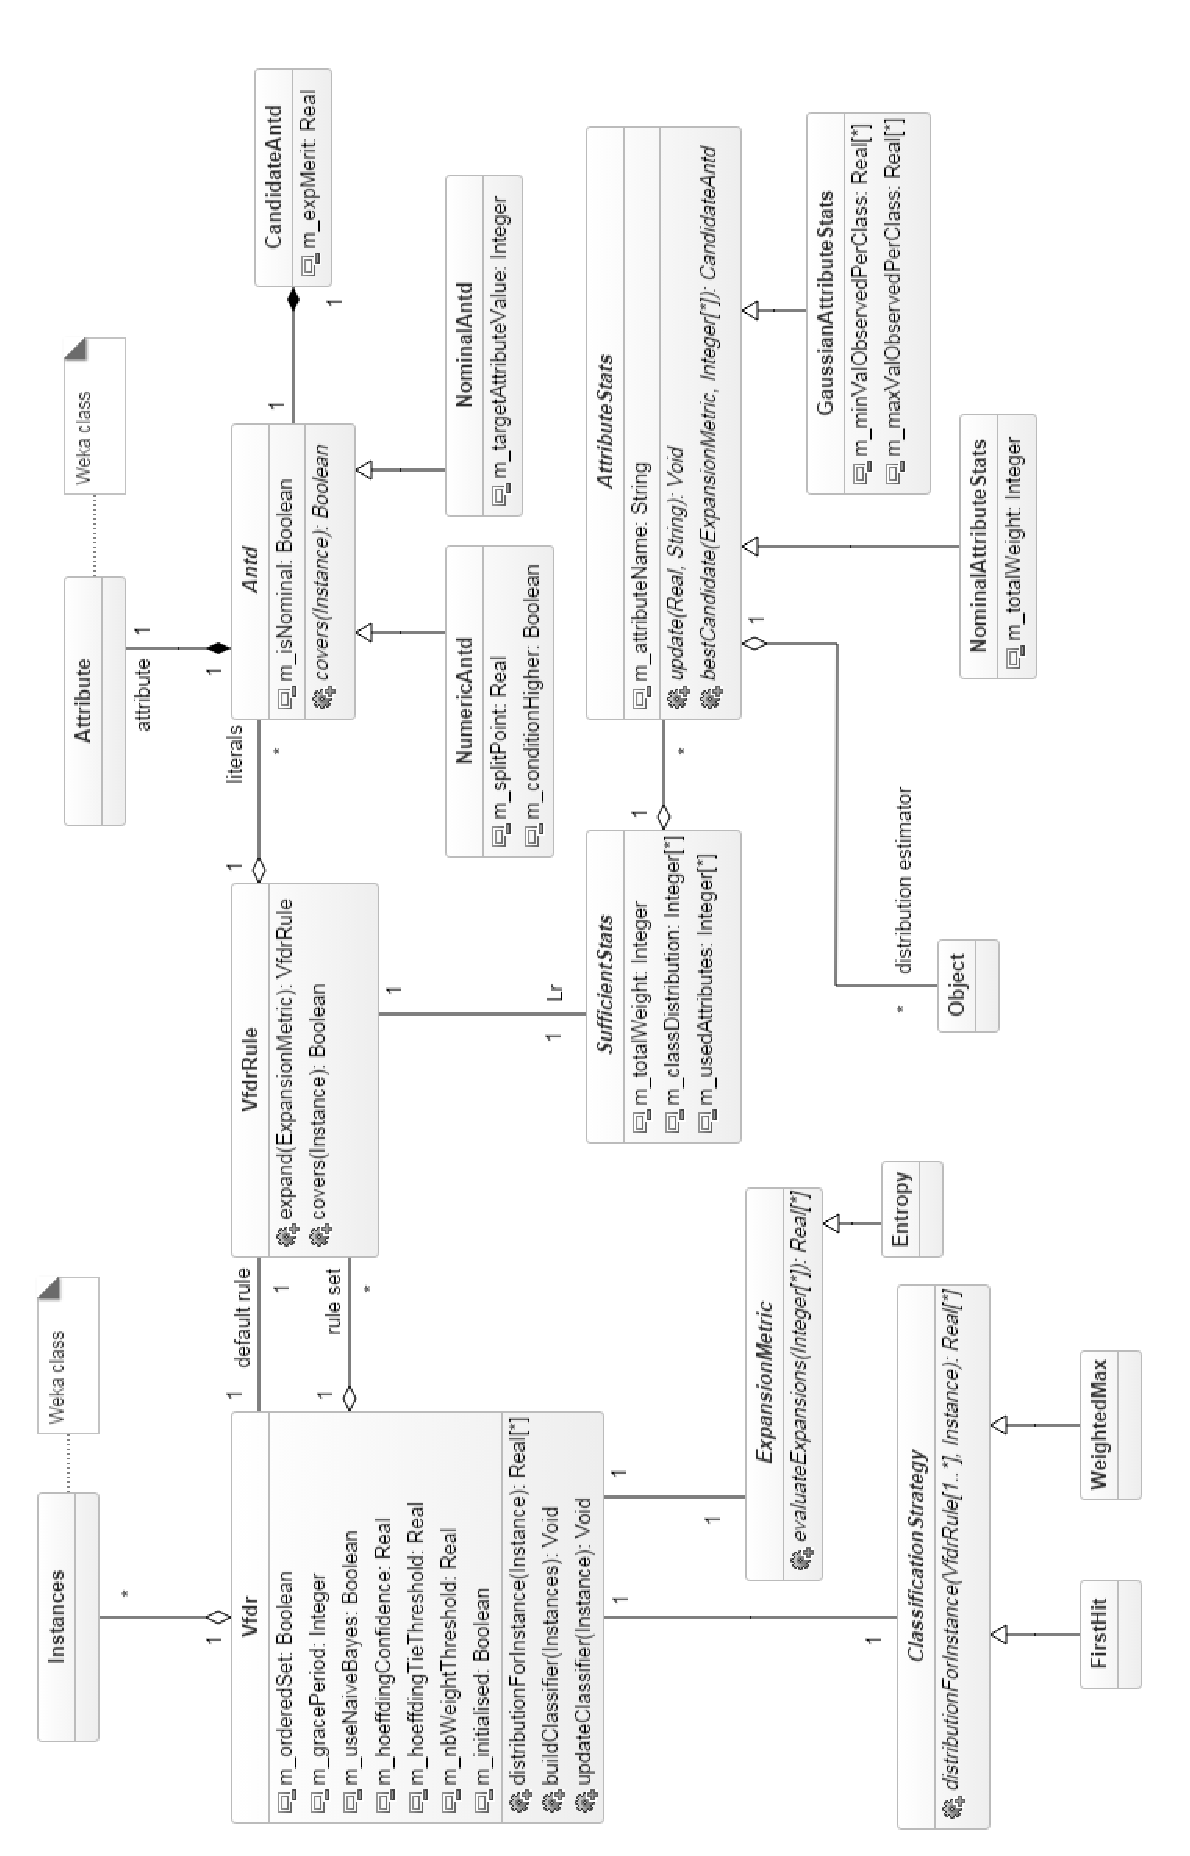
\includegraphics[width=\textwidth]{SOURCES/image2}

    \end{figure}


    \subsection{Description de l'implémentation}

        \paragraph{Paramétrage} La classe principale de notre programme, nommée \texttt{Vfdr}, implémente plusieurs interfaces de Weka, notamment UpdateableClassifier, qui permet de mettre en avant l’aspect incrémental de l’algorithme. Ces interfaces permettent d'intégrer le programme au GUI de Weka. \texttt{Vfdr} possède des attributs servant d’options de configuration, ainsi qu’une liste de \texttt{VfdrRule}, représentant l’ensemble des règles, et une \texttt{VfdrRule} à part, qui est la règle par défaut.

        \paragraph{Règles}Chaque objet \texttt{VfdrRule} possède lui-même une liste d’\texttt{Antd}, une classe abstraite servant à représenter les antécédents possibles pour les règles (spécialisée en \texttt{NumericAntd} pour les conditions sur les attributs numériques, et \texttt{NominalAntd} pour les conditions sur les attributs nominaux). \texttt{VfdrRule} possède aussi une référence vers un objet \texttt{SufficientStats}, qui stocke les statistiques associées à la règle. 


        \paragraph{Statistiques suffisantes} 
            Dans l’implémentation, nous avons choisi d’identifier les classes des exemples par des Strings (le nom de la classe). Par conséquent, dans \texttt{SufficientStats}, le nombre d’exemples couverts par classe est stocké dans une \texttt{Map<String, Integer>}. Pour ce qui est des attributs, ils peuvent être représentés par des entiers (leur indice). On utilise par exemple une \texttt{List<Integer>} pour stocker les attributs déjà utilisés dans \texttt{SufficientStats}. Cependant, les attributs sont parfois identifiés par leur nom, comme les classes : les statistiques par attributs sont stockés dans une \texttt{Map<String, \texttt{AttributeStats}>}, où \texttt{AttributeStats} est une classe abstraite qui a des spécialisations différentes selon le type d’attribut.
            
            Pour gérer les statistiques des attributs numériques, certaines descriptions de \texttt{VFDR} indiquent d’utiliser un arbre binaire qui stocke pour chaque attribut la chance de rencontrer une valeur supérieure à chaque valeur déjà rencontrée. Pour simplifier l’implémentation, nous avons plutôt utilisé une densité de probabilité pour représenter les valeurs rencontrées : c’est la classe \texttt{GaussianAttributeStats}, qui hérite de \texttt{AttributeStats}. Les calculs sont faits dans la classe interne \texttt{GaussianEstimator}, qui hérite de la classe Weka \texttt{UnivariateNormalEstimator}. Ce choix a aussi l’avantage de limiter la complexité en temps et en espace.
        
        \paragraph{Expansion d'une règle} Pour l’expansion d’une règle, une liste de \texttt{CandidateAntd} (antécédents candidats) est créée. Le score de chaque candidat est évalué à l’aide d’un objet \texttt{ExpansionMetric}. Notons qu’\texttt{ExpansionMetric} est une classe abstraite, mais qu’elle n’a qu’une seule spécialisation possible : \texttt{Entropy}, qui utilise des calculs d’entropie pour évaluer la qualité d’une séparation. La mise en place d’une classe abstraite permet de laisser la possibilité d’améliorer l’implémentation, en ajoutant des méthodes d’évaluation de séparation, en limitant les modifications à apporter au code existant.
        
        \paragraph{Prédiction} Lorsque l’on demande au \texttt{Vfdr} de classifier un exemple via la méthode \texttt{distributionForInstance}, sa stratégie de classification (représentée par la classe abstraite ClassificationStrategy) entre en jeu. Pour les ensembles ordonnés de règles, la stratégie est de type FirstHit, on renvoie la classe donnée par la première règle qui couvre l’exemple. Pour les ensembles non ordonnés, la stratégie est de type WeightedMax, on choisit alors la classe à partir de la règle qui couvre l’exemple et a le poids le plus élevé (le plus grand nombre total d’exemples couverts).

    \section{Third chapter}
        

    \section{Conclusion} 
%        \lipsum[2]

    \nocite{*}
    \bibliography{biblio}


\end{document}
